\documentclass[a4paper,UKenglish]{oasics}

\usepackage{microtype}%if unwanted, comment out or use option "draft"
\usepackage{amsmath}
\usepackage{amsfonts}
\usepackage{algorithm}
\usepackage{hyperref}
\usepackage[noend]{algpseudocode}
\usepackage{todonotes}
\usepackage{bbm}

\usepackage{listings}
\usepackage{color}

\definecolor{codegreen}{rgb}{0,0.6,0}
\definecolor{codegray}{rgb}{0.5,0.5,0.5}
\definecolor{codepurple}{rgb}{0.58,0,0.82}
\definecolor{backcolour}{rgb}{0.95,0.95,0.92}

\lstdefinestyle{mystyle}{
    backgroundcolor=\color{backcolour},
    commentstyle=\color{codegreen},
    keywordstyle=\color{magenta},
    numberstyle=\tiny\color{codegray},
    stringstyle=\color{codepurple},
   % basicstyle=\footnotesize,
    breakatwhitespace=false,
    breaklines=true,
    captionpos=b,
    keepspaces=true,
    numbers=left,
    numbersep=5pt,
    showspaces=false,
    showstringspaces=false,
    showtabs=false,
    tabsize=2
}

\lstset{style=mystyle}

\newcommand{\argmin}{\operatornamewithlimits{argmin}}


\graphicspath{{./images/}}

\bibliographystyle{plain}

% Author macros::begin %%%%%%%%%%%%%%%%%%%%%%%%%%%%%%%%%%%%%%%%%%%%%%%%
\title{Hey there's DALILA: a DictionAry LearnIng LibrAry}
\titlerunning{DALILA: A DictionAry LearnIng LibrAry}

\author[1]{Veronica Tozzo}
\author[1]{Vanessa D'Amario}
\author[1]{Annalisa Barla}
\affil[1]{Department of Informatics, Bioengineering, Robotics and System Engineering
(DIBRIS), University of Genoa\\ Genoa, I-16146, Italy\\
\href{mailto:\{veronica.tozzo, vanessa.damario\}@dibris.unige.it}{\{veronica.tozzo, vanessa.damario\}@dibris.unige.it} \\
\href{mailto:annalisa.barlao@unige.it}{annalisa.barla@unige.it}}
\authorrunning{V. Tozzo, V. D'Amario and A. Barla}%mandatory.

\Copyright{Veronica Tozzo and Vanessa D'Amario}%mandatory. OASIcs license is "CC-BY";  http://creativecommons.org/licenses/by/3.0/

\subjclass{G.1.6 Optimization, D.1.3 Concurrent Programming, D.2.2 Design Tools and Techniques}  %please refer to \url{http://www.acm.org/about/class/ccs98-html}}% mandatory: Please choose ACM 1998 classifications from http://www.acm.org/about/class/ccs98-html . E.g., cite as "F.1.1 Models of Computation".
\keywords{Machine learning, dictionary learning, representation learning, alternating proximal gradient descent, parallel computing}% mandatory: Please provide 1-5 keywords
% Author macros::end %%%%%%%%%%%%%%%%%%%%%%%%%%%%%%%%%%%%%%%%%%%%%%%%%

%Editor-only macros:: begin (do not touch as author)%%%%%%%%%%%%%%%%%%%%%%%%%%%%%%%%%%
\serieslogo{}%please provide filename (without suffix)
\volumeinfo%(easychair interface)
  {Billy Editor and Bill Editors}% editors
  {2}% number of editors: 1, 2, ....
  {Conference/workshop/symposium title on which this volume is based on}% event
  {1}% volume
  {1}% issue
  {1}% starting page number
\EventShortName{}
\DOI{10.4230/OASIcs.xxx.yyy.p}% to be completed by the volume editor
% Editor-only macros::end %%%%%%%%%%%%%%%%%%%%%%%%%%%%%%%%%%%%%%%%%%%%%%%

\begin{document}

\maketitle

\begin{abstract}
Dictionary Learning and Representation Learning are machine learning methods for decomposition, denoising and reconstruction of data with a wide range of applications such as text recognition, image processing and biological processes understanding. In this work we present DALILA, a scientific Python library for regularised dictionary learning and regularised representation learning that allows to impose prior knowledge, if available.
DALILA, differently from the others available libraries for this purpose, is flexible and  modular. DALILA is  designed to be easily extended for custom needs. Moreover, it is compliant with the most widespread ML Python library and this allows for a straightforward usage and integration.
We here present and discuss the theoretical aspects and discuss its strength points and
implementation.
%The library is implemented in Python and it is publicly available for download at github link \texttt{https://github.com/slipguru/dalila} or via pip and conda install. The library is presented with example and documentation.
\end{abstract}


\section{Introduction}
%Dictionary learning is a decomposition method that, given a data matrix, finds two new matrices: one of basic signals, the dictionary, and one of their relative weight, the so called coefficients. In Representation Learning, instead, the dictionary is given and the problem is to find the coefficients that better approximate the data.
%
%Due to their unsupervised nature and to their minor spread, fewer implementations for DL and SC with respect to other tasks are accessible.

%Matrix decomposition is
Nowadays many optimisation algorithms and libraries are freely available for the most disparate machine learning applications. For example some machine learning tasks, as classification, have hundreds of algorithms and libraries implementations. This is not the case for \emph{Dictionary Learning} (DL) \cite{lee1999learning, lin2007,  Mairal2010, mairal2009supervised,  rakotomamonjy2013direct, salzo2014alternating, tosic2011dictionary} and its specialisation \emph{Representation Learning} (RL) \cite{6472238, 4385788}, which are designed for matrix decomposition and reconstruction.
They can be applied on many application domains such as signal processing \cite{tosic2011dictionary}, image processing \cite{ravishankar2011mr}, bioinformatics \cite{alexandrov2013deciphering} and text-recognition \cite{aggarwal2012mining}. Even though dimensionality reduction methods such as PCA \cite{jolliffe2002principal} and ICA \cite{hyvarinen2004independent} may be used to solve these tasks, dictionary learning is preferable when more emphasis on the interpretability of the dictionary is required  \cite{lee1999learning}. %, \textcolor{red}{see \cite{lee1999learning} for more details about the comparison of the methods}.

In this paper we present DALILA, a Python library for DL and RL. The optimisation is based on \emph{alternating proximal gradient descent} \cite{bolte2014proximal}, which allows flexibility on the minimisation problem and therefore enables the imposition of prior knowledge.
Designed to be extremely flexible and modular, DALILA can be easily extended differently from the other available libraries.

As regards the implementation, the library is compatible with the \texttt{scikit-learn} Python library and it supports the distribution of the most computationally heavy routines across different machines \cite{dask}.%; moreover the most computationally heavy routines of the library can be optionally distributed greatly reducing the total wall-clock time.

The remainder of this paper is organised as follows. In Section \ref{background} we present DL, RL and the alternating proximal gradient descent algorithm. In Section \ref{codesec} we give an overview on the library design and the implemented regularisers. In section \ref{related work} we comment the other available libraries on the topic. We finish with the conclusion and further work we intend to perform.



\section{Theoretical background} \label{background}

In the following section a basic theoretical background on DL and RL problems is provided, together with the alternating proximal minimisation algorithm. The expert reader can feel free to skip it, if she/he is familiar with these mathematical concepts.
% we introduce definition and functions
%Let us first define the notation we use. Bold upper case letters as $\textbf{X}$ denote matrices, whose $i$-th row is indicated as $\textbf{X}_{i,:}$ and $j$-th column as $\textbf{X}_{:,j}$. The generic element of the matrix $\textbf{X}$ is denoted by $x_{ij}$. Single vectors are written as bold lower case letters $\textbf{v}$.


\subsection{Dictionary Learning}
Dictionary learning (DL) is a machine learning method that aims at finding a representation of the original data as a linear combination of basic patterns (atoms) and coefficients. The representation is completely data driven, in contrast to more generic and less adaptive methods such as Wavelet and Fourier transform \cite{mallat2008wavelet, vetterli2013fourier}.

Given a dataset $\textbf{X} \in \mathbb{R}^{n\times d}$ where $n$ is the number of samples and $d$ is the feature space dimension, the goal of DL is to decompose a dataset into two matrices:
\begin{itemize}
\item a dictionary $\textbf{D} \in \mathbb{R}^{k\times d}$, a matrix of atoms that represent basic signals;
\item the coefficients $\textbf{C} \in \mathbb{R}^{n\times k}$, a matrix of weights for the atoms of the dictionary.
\end{itemize}
$k$ represents the number of atoms composing the dictionary.%, whose choice is a critical point of this problem and will be discussed later on.

Hence, the original matrix $\textbf{X}$ can be retrieved as a linear combination of dictionary and coefficients as in Equation (\ref{linear combination}).
\begin{equation}\label{linear combination}
\textbf{X} \approx \textbf{C}\textbf{D}
\end{equation}
The recovering of the matrices $\textbf{C}$ and $\textbf{D}$ is solved by minimising a loss term $\ell$: a a positive differentiable function that quantifies how well the multiplication of the two matrices approximates the signal.
\begin{equation}\label{loss function}
\underset{\textbf{C}, \textbf{D}}{\text{argmin}}\bigg[\ell(\textbf{X}, \textbf{C} \textbf{D}) \bigg]
\end{equation}

The minimisation problem in Equation (\ref{loss function}) not always gives us the best possible solution. In presence of noisy data, ill-posed problems or when we have prior knowledge on the problem one of the usual tricks is to add terms or constraints to the functional in order to obtain a regularised problem (Equation (\ref{generic functional})).
%
%The formalisation of this regularised problem is given in Equation (\ref{generic functional}).
\begin{equation}\label{generic functional}
\underset{\textbf{C}, \textbf{D}}{\text{argmin}} \bigg[ \ell(\textbf{X}, \textbf{CD}) + \Phi(\textbf{C}) + \Psi(\textbf{D}) \bigg]
\end{equation}
%\bigg[\sum_{i=1}^N  (\ell(\textbf{X}_{i,:}, \textbf{C}_{i,:}, \textbf{D}) + \Phi(\textbf{C}_{i,:})) + \sum_{j=1}^k \Psi(\textbf{D}_{j,:})\bigg]
$\Phi(\textbf{C})$  and $\Psi(\textbf{D})$ are two penalty functions that act respectively on the coefficients and on the dictionary.
The functional in Equation (\ref{generic functional}) can be further specialised in order to include constraints sets that reduce the space in which a solution is admissible. A very common example is when we impose the involved matrices to be non-negative, a problem known as Non-negative Matrix Factorization (NMF) \cite{lee1999learning}.
%
%
\subsection{Alternating proximal gradient descent}
It is worth noting that the optimisation of Equation (\ref{generic functional}) poses some issues. In fact, due to the multiplication present in the loss function $\ell$, Equation (\ref{generic functional}) is jointly non-convex. Moreover the generality of the penalty terms requires the use of a minimisation algorithm that deals with different choices of penalties without a substantial change in its flow.

All taken into account, our optimisation choice is \emph{alternating proximal gradient descent} \cite{bolte2014proximal} which assures the convergence to a local minima under the following assumptions: 1) the loss function $\ell(\textbf{X}, \textbf{C}\textbf{D})$  is differentiable and partially Lipschitz continuous; 2) it is possible to compute the proximal mapping of the penalty terms in closed form or at least to approximate it. See \cite{bolte2014proximal} for mathematical details and theoretical proofs.

The proximal mapping \cite{parikh2014proximal} of a function $g$ for a point $\textbf{u}$ is defined as Equation (\ref{proximal mapping}).
\begin{equation}\label{proximal mapping}
\text{prox}_{\mu g}(\textbf{u}) = \underset{\textbf{v}}{\text{argmin}}\left(g(\textbf{v}) + \frac{1}{2\mu}\parallel\textbf{v} - \textbf{u}\parallel_2^2\right)
\end{equation}
%which, roughly speaking, means that you are looking for a point that minimises $g$ and it is close to $\textbf{u}$.
When the computation of the prox is not available in a closed form, it can be approximated via a iterative algorithm.

A general overview on the optimization algorithm is given in Algorithm  \ref{altprox}. The algorithm alternates the steps 3, 4, 5 and 6 until convergence. In step 4 the computation of the gradient descent is performed on the dictionary keeping the coefficients fixed. On the result the proximal mapping of the dictionary learning penalty $\Psi$ is applied. The same is done in step 6 on the coefficients.

We want to remark that the gradient is computed w.r.t. the previous iteration in both cases \cite{rakotomamonjy2013direct}. This allows to perform the two steps in parallel if needed.

\begin{algorithm}[H]
\caption{Alternating proximal gradient descent}\label{altprox}
\begin{algorithmic}[1]
\State $\text{Random initialization of the matrices}\ C\ \text{and}\ D$
%\State $\text{Let} \ \mathcal{F} \text{ be the name of } {\parallel}X - CD{\parallel}_F^2$
\For {$i=0:\text{max{\_}iters}$}
\State $\gamma_D \gets \text{lipschitz\_step}_\ell(D)$
\State $\gamma_C \gets \text{lipschitz\_step}_\ell(C)$
\State $D_{t+1} = \text{prox}_{\gamma_D \Psi}(D_t - \gamma_D \bigtriangledown_D(\ell_t))$
\State $C_{t+1} = \text{prox}_{\gamma_C \Phi}(C_t - \gamma_C \bigtriangledown_C(\ell_t))$
\If{$\text{difference between iterates}< \epsilon\ \textbf{and}$\\
 \qquad $\ \ \text{different between previous and current objective function}<  \epsilon$}
\State $\textbf{break}$
\EndIf
\EndFor
\end{algorithmic}

\end{algorithm}
%
%
\subsection{Representation learning (sparse coding)}
Representation learning is a more general form of sparse coding (SC) that similarly to DL aims at finding the best approximation of a signal $\textbf{X}$ (Equation (\ref{linear combination})), when the dictionary $\textbf{D}$ is given. This leads to a problem which is easier to minimise and, given convex loss function and penalty, becomes convex.
The convexity property guarantees that a global optimum can be always reached.

In representation learning the choice of the penalty on the coefficients is arbitrary and dictated by the problem while in SC we assume the use of $L^0$ or $L^1$ norms. The formalisation is given in Equation (\ref{sparse coding}).
\begin{equation}\label{sparse coding}
\underset{\textbf{C}}{\text{argmin}} \bigg[ \ell(\textbf{X}, \textbf{CD}) + \Phi(\textbf{C}) \bigg]
\end{equation}
This optimisation problem, since involves the minimisation on only one variable, can be solved with proximal gradient descent that acts similarly to what explained in Algorithm \ref{altprox} without steps 3 and 5.
%
%


%The tuning of the parameter can be further improved by shrinking the interval toward those parameters that give a better cross-validation result.



\section{DALILA}\label{codesec}
DALILA is a library for signal decomposition and reconstruction. Its first focus is Dictionary Learning (DL) described in Section \ref{background}. The fact that both the dictionary and the coefficients are learned from data allows for a more complete analysis of the results  extracting useful information about the original signals. Moreover the possibility to impose prior knowledge on the problem using penalty terms grants that the final matrices respect certain constraints.
Examples for regularised DL are: 1) image denoising where sparsity imposition forces the most important atoms to be used and the noisy ones to be discarded; 2) pattern recognition, where the atoms of the dictionary are seen as latent patterns from which the original signals are generated.

DALILA second focus is Representation Learning whose purpose is to represent the original data matrix on a new space defined by the atoms of the dictionary $\mathbf{D}$. Penalty terms can be added to impose a structure on this new representation.

The learned coefficients may be used as a new representation for further tasks such as: 1) compressed sensing that exploits sparsity reducing the size of the original signal; 2) classification where, rather than considering the original signal, the coefficients are used as new features.

\begin{figure}[!h]
\centering
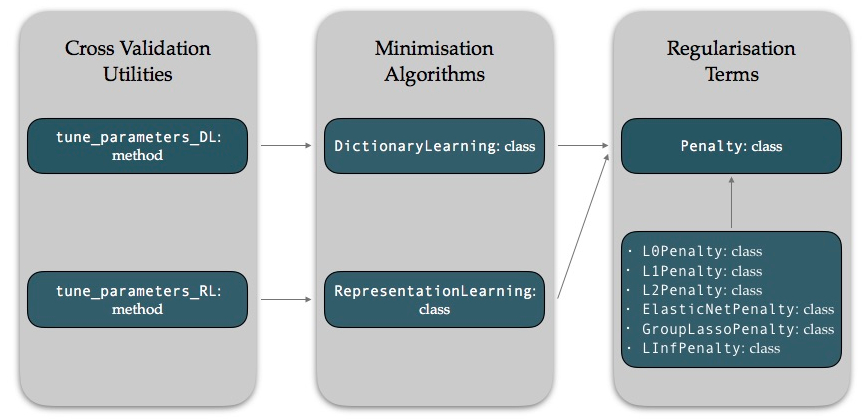
\includegraphics[width=0.9\textwidth]{schema}
\caption{Diagram of DALILA library structure.
The main core consists of the two classes which address the minimization problem.
This depends on the class Penalty which represents a generic penalty term and that can be specialised by declaring subclasses.
 The library also offers cross validation utilities for the free parameters tuning. }
\label{schema}
\end{figure}

\subsection{Implementation}
DALILA is implemented in Python. It supports different versions of Python and it is \texttt{scikit-learn} compatible. See \url{https://slipguru.github.io/dalila} for the full documentation and a quick start.

DALILA has a modular and easily extendible design (see Figure \ref{schema}). The core of the library consists of two classes,  \texttt{DictionaryLearning} and \texttt{RepresentationLearning} which respectively solve the two minimisation problems in Equation (\ref{generic functional}) and (\ref{sparse coding}). These classes depend on a generic penalty term (\texttt{Penalty}) which can be specialised into different regularisers by declaring a subclass. The library is therefore easily extendible with new regularisers and flexible in the choice of the model.
Cross validation utilities to tune the parameters of the model are provided, the two methods shown in Figure \ref{schema}, \texttt{tune\_parameters\_DL} and \texttt{tune\_parameters\_RL}, can perform the tuning by parallel or distributed computation using \texttt{dask} library \cite{dask}.\\

%\textcolor{red}{In the library the loss function $\ell$, introduced in a generic form in Equation (\ref{generic functional}) and (\ref{sparse coding}), is commong to both \texttt{DictionaryLearning} and \texttt{RepresentationLearning} classes and it is the Frobenius norm of the difference between the original signal and its reconstruction, defined as Equation (\ref{square loss}).}

The loss function $\ell$ introduced in a generic form in Equation (\ref{generic functional}) and (\ref{sparse coding}) is common to both \texttt{DictionaryLearning} and \texttt{RepresentationLearning} classes.
It is implemented as the Frobenius norm of the difference between the original signal and its reconstruction, defined as Equation (\ref{square loss}).
\begin{equation}\label{square loss}
\ell(\textbf{X}, \textbf{CD}) = \|\textbf{X} - \textbf{CD}\|_F^2
\end{equation}

As regards the regularisation terms, called $\Phi$ and $\Psi$ in Equation (\ref{generic functional}) and (\ref{sparse coding}),  DALILA
offers many possibilities.
%The implementation of %as \texttt{L1Penalty}, \texttt{L2Penalty}, \texttt{ElasticNetPenalty}, \texttt{GroupLassoPenalty},
%\texttt{LInfPenalty} and \texttt{L0Penalty} (described in Section \ref{penaltiessec}) is provided.
In this way a proper regulariser, dependent from the task, can be chosen, during the initialisation of the \texttt{DictionaryLearning/RepresentationLearning} instances.
In fact \texttt{DictionaryLearning/RepresentationLearning} minimisation algorithms do not depend on the penalties chosen,
as long as the penalty classes inherit from the superclass \texttt{Penalty} and reimplement the same methods (Figure \ref{schema}).
For a better understanding see Appendices \ref{penalty change}, \ref{new penalty}.
\paragraph*{Available regularisation terms}\label{penaltiessec}
%\textcolor{red}{The penalty terms in the library refer to the ones introduces in Equation (\ref{generic functional}) and (\ref{sparse coding}), $\Phi$ and $\Psi$. We now explain some of the possible choices and their properties.}

The penalty terms $\Phi$ and $\Psi$ are the product between a regularisation parameter and, typically, a norm. The norm is used to impose a structure on the matrix, while the regularisation parameter, a positive scalar, weights the regularisation term influence on the solution.%regularised the solution should be.
%All the penalties we present here are applied by row because of the structure of the matrices: on the rows of coefficients matrix lie the samples while on the rows of the dictionary matrix lie the atoms.

In the following we show the possible choices for $\Phi$ and $\Psi$ applied on a generic matrix $\textbf{M}$ whose $i$-th row is indicated as $\textbf{M}_{i,:}$ and $j$-th column as $\textbf{M}_{:,j}$. Its generic element is denoted by $m_{ij}$. With the notation $\Phi|\Psi$ we indicate that the penalty can be applied or on the dictionary or on the coefficients or on both.\\
\begin{itemize}
%
%
%
\item \texttt{L1Penalty} - \textbf{$\ell_1$ norm}
\begin{equation}\label{l1penalty}
\Phi|\Psi(\mathbf{M}) = \lambda \sum_i \|\mathbf{M}_{i,:}\|_1 =  \lambda \sum_i \sum_j |m_{ij}|
\end{equation}
Regularisation terms of this form, due to the geometrical meaning of the $\ell_1$ norm, force the solution to be sparse and, therefore, highly interpretable \cite{tibshirani1996regression}. If the penalty is applied on the dictionary it promotes a dictionary whose atoms have a low number of non-null components. For the coefficients, the penalisation promotes a reconstruction based only on few atoms of the dictionary, discarding the ones which give minor contribution to the original signal.

The proximal operator related to this regulariser is
\begin{equation}\label{proxl1}
\text{prox}_{\Phi|\Psi}(m_{ij}) =
\begin{cases}
       m_{ij} - \lambda &\text{ if }m_{ij} > \lambda \\
       0 & \text{ if }m_{ij} \in [-\lambda, \lambda] \\
       m_{ij} + \lambda & \text{ if }m_{ij} < -\lambda
\end{cases}
\end{equation}
%
%
%
\item \texttt{L2Penalty} - \textbf{$\ell_2$ norm}
\begin{equation}\label{l2penalty}
\Phi|\Psi(\mathbf{M}) = \lambda \sum_{i}\left({\sum_j m_{ij}^2}\right)^\frac12
\end{equation}

Penalties of this form, as in the previous case, can be applied to both matrices $\mathbf{C}$ and $\mathbf{D}$.
The $\ell_2$ regularisation term leads to the shrinkage of the components of each row, but, differently from the $\ell_1$ norm, it does not lead to a sparse solution \cite{tikhonov1977solutions}.

The proximal operator is
\begin{equation}\label{proxl2}
\text{prox}_{\Phi|\Psi}(\mathbf{M}_{i,:}) = \text{max}(1 - \lambda/ \| \mathbf{M}_{i,:}\|_2, 0)\ \mathbf{M}_{i,:}
\end{equation}
%
%
%
\item \texttt{ElasticNetPenalty}
\begin{equation}\label{l1l2penalty}
\Phi|\Psi(\mathbf{M}) = \sum_{i}\bigg[\alpha \lambda_1 \|\mathbf{M}_{i,:}\|_1 + (1 - \alpha)\lambda_2 \|\mathbf{M}_{i,:}\|_2 \bigg]
\end{equation}
Elastic Net can be preferable to $\ell_1$ norm, in the case of highly correlated variables, and also to $\ell_2$ norm since it inherits the possibility of finding a sparse solution \cite{zou2005regularization}.

Here $\lambda_1$ and $\lambda_2$ weight the two norms separately while $\alpha \in [0,1]$ balances the contribution of the two terms. The proximal operator is

\begin{equation}\label{proxen}
\text{prox}_{\Phi|\Psi}( \mathbf{M}_{i,:}) = \left(\frac{1}{1 + \alpha\lambda_2}\right) \text{prox}_{\lambda_1 \|\cdot\|_1} ( \mathbf{M}_{i,:})
\end{equation}
%
%
\item \texttt{L0Penalty} - \textbf{$\ell_0$ pseudo-norm}
\begin{equation}\label{l0penalty}
\Phi|\Psi(\mathbf{M}) : \forall i\ \    \|\mathbf{M}_{i,:}\|_0 \leq s
\end{equation}
where $\|\mathbf{M}_{i,:}\|_0$ counts the number of non-zero elements in the row. The regularisation parameter $s\in \mathbb{N}$ impose the maximum number of non-null elements in $\mathbf{M}_{i,:}$, naturally leading to sparse results. The proximal operator is
\begin{equation}
\text{prox}_{\Phi|\Psi}(\textbf{M}_{i,:}) = \begin{cases} &m_{ij}, \text{ if } m_{ij} \in \mathcal{S} \\ &0, \text{ otherwise} \end{cases}
\end{equation}
where $\mathcal{S}$ is the set containing the first $s$ biggest components of $\textbf{M}_{i,:}$.\\
%
%
%\item \textbf{TVL1Penalty} This term is the sum of two regularisations, Total Variation (TV) and $L^1$ norm, that act row-wise on the matrix. It is formalised as:
%\begin{equation}\label{linfpenalty}
%\text{TV-L1}(\mathbf{M}) = \sum_i \left[\lambda_{TV} \sum_j  |\mathbf{M}_{i,j} -\mathbf{M}_{i,j-1}| + \lambda_1 \|\mathbf{M}_{i,:}\|_1 \right]
%\end{equation}
%The two regularisation parameters act on the different part of the penalty in order to put more emphasis on one of the two parts. The penalty forces the row of the matrix to be piece-wise constant and to have few parts different from zero.
%
%Its proximal cannot be computed in closed form but requires an approximation. The algorithm we chose is the one presented in \cite{salzo2014alternating} which is able to approximate the prox up to a precision $\epsilon$ set by the user. \\
%%
%%
%%
\item \texttt{LInfPenalty} - \textbf{$\ell_\infty$ norm}
\begin{equation}\label{linfpenalty}
\Phi(\mathbf{M}) = \lambda \sum_j \|\mathbf{M}_{:,j}\|_\infty
\end{equation}
where $\|\mathbf{M}_{:,j}\|_\infty$ returns the maximum element in the column.
This regularisation term acts column-wise only on the coefficients and it is useful in presence of a redundant dictionary \cite{tropp2006just}.

The effect of this regulariser is to discard the atoms that overall have a low impact in the reconstruction while emphasising the atoms that, even if only in few samples, contribute largely.

The proximal operator is
\begin{equation}\label{proxlinf}
    \text{prox}_{\Phi}(\mathbf{m}_j) = \mathbf{m}_j - \lambda \Pi_1(\mathbf{m}_j/\lambda)
\end{equation}
The algorithm for the projection on the $\ell_1$ ball is explained in \cite{duchi2008efficient}.\\
%
%
%
\item \texttt{GroupLassoPenalty} - \textbf{$\ell_{1,2}$ norm}
\begin{equation}\label{group lasso penalty}
\Phi|\Psi(\mathbf{M}) = \lambda \sum_i \sum_{g \in \mathcal{G}} \|\mathbf{M}_{i,g}\|_2
\end{equation}
where $\mathcal{G}$ is the set of the groups (i.e. the indices of the columns) defined by the user.

For each row of the matrix $\mathbf{M}$ the penalty enforces all the values of a group to be selected or discarded together (i.e. all of them set to zero). The groups cannot be overlapping and they have to cover all the columns indices.
Its proximal mapping is
\begin{equation}\label{proxgrouplasso}
    \text{prox}_{\Phi|\Psi}(\mathbf{M}_{i,:})_\mathcal{G} = \text{max}(1 - \lambda/ \| \mathbf{M}_{i,g}\|_2, 0)\ \mathbf{M}_{i,g} \ \ \text{for all } g \in \mathcal{G}
\end{equation}

\item \textbf{Additional user-implemented penalties}
As introduces before DALILA is flexible in the sense that it allows to use different penalties without changing the minimisation
 flow and it further allows the user to declare new non-considered penalties. More details are given in Appendix \ref{new penalty}. 
\end{itemize}

\vspace{0.5cm}
Both for \texttt{DictionaryLearning} and \texttt{RepresentationLearning} the user can impose non-negativity constraints on the involved matrices.
When this requirement is applied both on the dictionary and the coefficients it is called Non-negative Matrix Factorization % and it useful when, for example, we are analysing images or biological data
\cite{lee1999learning}.
%, alexandrov2013deciphering}.
The non-negativity condition can, moreover, be imposed only on the coefficients in order to obtain a more
interpretable contribution of the dictionary elements to the reconstruction of the original signal \cite{salzo2014alternating}. The projection is performed
by setting to zero all the negative elements in the considered matrix.
%
%

Furthermore, in the \texttt{DictionaryLearning} class the user can impose the
normalization condition on the dictionary matrix, which is equivalent to set the euclidean norm of each row equal to 1.
\begin{equation}\label{dictionary normalisation}
\|\mathbf{D}_{i,:}\|_2 = 1\ \ \text{for all }i \in \{1, \dots, k\}
\end{equation}

%\\Concerning \texttt{DictionaryLearning} non-negativity can be imposed on both matrices, on the coefficients or on none of them, while for \texttt{RepresentationLearning} the non-negativity is a boolean flag.
%\subsection{Projections}\label{projections}
%In addition to all the penalties it is possible to perform two projections:


%
%\section{Model selection}
%
%
%A common technique employed for this purpose is \emph{cross-validation}, a model validation method which assesses how well a model performs over a certain finite set of parameters sampled from an interval. Since the search can be done on multiple parameters at the time the best combination is chosen by inspecting the mean goodness score of the model.
%
%Since Dictionary Learning is an unsupervised problem we use the



%DictionaryLearning further exposes an $L^2$-ball projection of ray 1.

%After initialisation of the objects it is possible to fit the estimators on a data matrix via (alternating) proximal gradient descent.
%Both DictionaryLearning and RepresentationLearning are implemented following the rules for the estimators of scikit-learn. This allows for using them in sklearn functions, an example is GridSearchCV that is used in the parameter research procedure.

\paragraph*{Model selection}
A critical aspect of these reconstruction techniques is constituted by the choice of the free parameters,
 which are the number of atoms $k$ that define the dictionary and the regularisation values that weight the penalty terms.
 This choice depends on the dataset given as input $\mathbf{X}$ and it can varies depending on different factors,
 as the high level of noise in the measurements, the redundancy of the founded dictionary and the interpretability
 of the solution. Given the fact that there is an infinite set of possible values for each parameter and no
 theoretical formulation that guides to the best solution exists, the only feasible approach is to empirically solve a searching problem over the parameters space.

DALILA allows for a fine tuning of the free parameters of the model on the dataset by performing a grid search based on cross validation. The best combination of parameters is selected as the one that returns the best mean score over multiple iterations. As score we use BIC (Bayesian Information Criterion) \cite{schwarz1978estimating}, shown in Equation (\ref{BIC}).
\begin{equation}\label{BIC}
\text{BIC} = - \text{log}(n)\cdot k - c \cdot \ell(\textbf{X},\textbf{CD})
\end{equation}
where $c$ is a positive constant. The highest value of the BIC corresponds to the best model in the search space.
This procedure is available both for \texttt{DictionaryLearning} and \texttt{RepresentationLearning}.

The two procedures, \texttt{tune\_parameters\_DL} and \texttt{tune\_parameters\_RL}, allow the user to specify different search modalities.
In \texttt{tune\_parameters\_DL} the user can choose among different configurations.
\begin{itemize}
\item tuning the number of atoms together with the dictionary penalty and after searching the regularisation parameter on the coefficients;
\item fixing the number of atoms in the estimator and tuning the penalties together;
\item fixing the penalties values and tuning the best number of atoms;
\item tuning all the possible value together, number of atoms and regularisation parameters, analysing every possible combination in the grid.
\end{itemize}

\section{Related work}\label{related work}
As of today other libraries addressing similar tasks are available, {SPAMS}\footnote{\url{http://spams-devel.gforge.inria.fr/doc/html/}} (SPArse Modeling Software) \cite{Mairal2010} and the Decomposition modules of scikit-learn \cite{cichocki2009fast, lin2007}.

SPAMS, implemented in C++, performs the  decomposition tasks through dictionary learning, non negative matrix factorization and sparse PCA. It offers a good set of options, but, even if it is interfaceable with Python, it is not \texttt{scikit-learn} compatible. Therefore, it cannot be integrated in \texttt{scikit-learn} pipelines. Moreover, it is non trivial to customise or extend it.

The other main competitor, the decomposition module of \texttt{scikit-learn} library, implements dictionary learning and NMF but it only has few fixed penalty terms.

\section{Conclusions and further work}

In this work we introduced DALILA, a library for dictionary learning and representation learning. We presented its main features: the wide variety of penalties, the possibility to customise the library on specific problems, its compatibility with \texttt{scikit-learn} library, its high flexibility and its scalable architecture which allows to perform parallel parameter searching procedures.

The wide variety of penalties applicable on the matrices allow the user to solve a broad range of problems. Moreover, since scientific problems can introduce more specific and new needs, the possibility to customise and adapt the library is essential.

DALILA is fully compliant with one of the most complete machine learning Python libraries that is \texttt{scikit-learn}. This makes almost effortless its integration with the majority of machine learning Python pipelines.

The possibility to parallelise or distribute computationally heavy routines \cite{dask}  greatly reduce the wall-clock time. Nevertheless our implementation is still basic and therefore the time performance are worse compared to the other presented libraries. In the future we plan to replace the use of \texttt{dask} with an hybrid parallelised system which will take advantage both of MPI tasks distribution and the computational acceleration given by GPUs. 

Given DALILA flexibility and the existence of other Dictionary Learning related problems, we aim at extending it. The planned expansions are: 1) Discriminative Dictionary Learning \cite{mairal2009supervised}, a variant of the dictionary learning problem which includes the classification task; 2) Shift Invariant Dictionary Learning \cite{grosse2012shift} that allows the reconstruction of signals using atoms with smaller support than the original signal and 3) Total Variation penalty in combination with Lasso \cite{salzo2014alternating}.

%\begin{lstlisting}[caption={Useless code},label=list:8-6,captionpos=t,float,abovecaptionskip=-\medskipamount]
%for i:=maxint to 0 do
%begin
%    j:=square(root(i));
%end;
%\end{lstlisting}


%
%\subparagraph*{Acknowledgements}
%
%Dobbiamo ringraziare qualcuno? Saverio per il supporto teorico?
%%
%% Bibliography
%%

%% Either use bibtex (recommended), but commented out in this sample
\bibliography{bib}

\newpage
\appendix

\section{Appendix: example of usage and related output}
In this appendix we want to offer some insights of how DALILA code works and the possible outcomes we can obtain. All the experiments are performed on the ORL database of faces \footnote{The database is available for download at the link \url{http://www.cl.cam.ac.uk/research/dtg/attarchive/facedatabase.html}}. This database is saved as a matrix within the library with 400 samples and $112\times 92$ features.

In order to perform Dictionary Learning on this dataset we firstly need to flatten the matrices into arrays and then apply the fitting procedure. In this estimator we are using an arbitrary number of atoms that we choose randomly and we impose non-negativity on both the matrices since we are dealing with gray scale images that have values in the range of [0,255]. 
\begin{lstlisting}[language=Python]
import numpy as np

from dalila.dictionary_learning import DictionaryLearning
from dalila.penalty import L1Penalty

dataset = np.load("/path/to/dalila/folder/dalila/databases/ORL_database.npy")
d1, d2, n = dataset.shape
data = np.empty((n, d1*d2))
for i in range(n):
	data[i,:] = np.ravel(dataset[:,:,i])

estimator = DictionaryLearning(k=60, non_negativity="both")
estimator.fit(data, n_iter=1000)
C, D = estimator.decomposition()
\end{lstlisting}
Some of the results obtained with this code are depicted in Figure \ref{atoms}. Here the most used atoms in the reconstructions are showed.  In Figure \ref{reconstructions}, instead, we show some reconstructions and their original signals to perform a qualitative comparison.
\begin{figure}[H]
\centering
\begin{tabular}{ccccc}
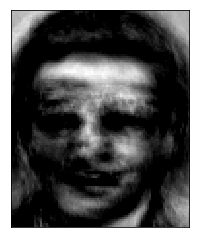
\includegraphics[scale=0.3]{atom_0.png} &
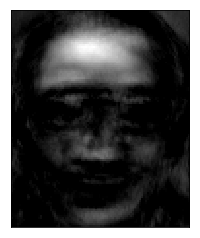
\includegraphics[scale=0.3]{atom_1.png} &
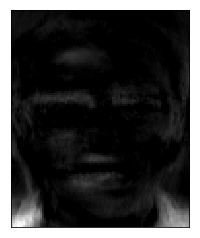
\includegraphics[scale=0.3]{atom_2.png} &
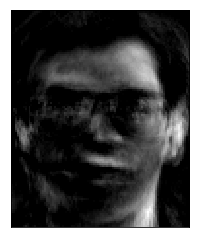
\includegraphics[scale=0.3]{atom_3.png} &
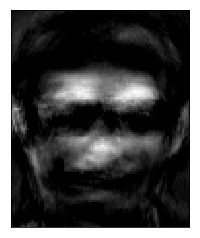
\includegraphics[scale=0.3]{atom_4.png} \\
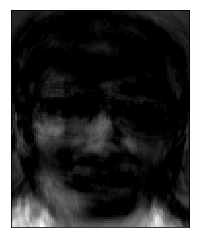
\includegraphics[scale=0.3]{atom_5.png} &
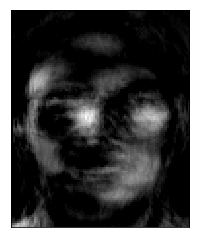
\includegraphics[scale=0.3]{atom_6.png} &
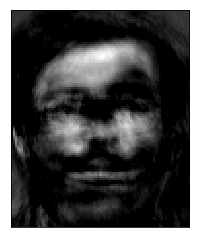
\includegraphics[scale=0.3]{atom_7.png} &
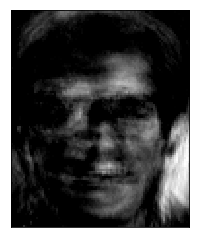
\includegraphics[scale=0.3]{atom_8.png} &
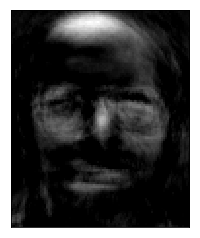
\includegraphics[scale=0.3]{atom_9.png} \\
\end{tabular}
\caption{The ten more recurrent atoms for the reconstruction of the samples in ORL dataset.}
\label{atoms}
\end{figure}

\begin{figure}[H]
\centering
\begin{tabular}{ccc}
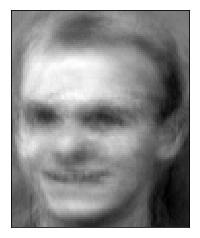
\includegraphics[scale=0.5]{reconstruction1.png} &
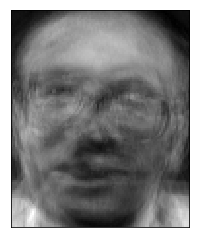
\includegraphics[scale=0.5]{reconstruction2.png} &
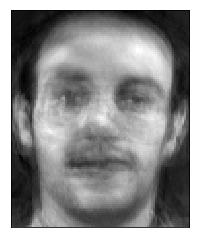
\includegraphics[scale=0.5]{reconstruction3.png}\\
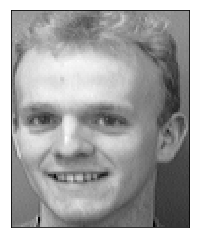
\includegraphics[scale=0.5]{original1.png} &
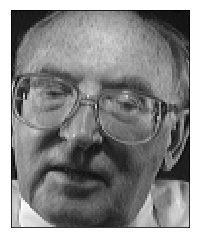
\includegraphics[scale=0.5]{original2.png} &
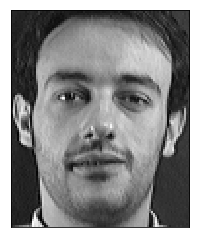
\includegraphics[scale=0.5]{original3.png}\\
\end{tabular}
\caption{Examples of the reconstruction obtained with DL decomposition. In the first row the reconstructions are shown and beneath them their original picture.}
\label{reconstructions}
\end{figure}


In this example we tune only the right number of atoms we should use for this particular dataset. Given the dimensionality of the dataset we picked as range $k \in [5,10,15,20,30,40,50]$. 

Moreover we did not use the basic BIC score but a normalised one since the values within the BIC computation, with this dataset, are not comparable in their magnitude (see \texttt{scoring\_function}). The results are showed in Figure \ref{bic} where we can see that the best number of atoms is 15.
\begin{lstlisting}[language=Python]
import matplotlib.pyplot as plt
import numpy as np
from dalila.parameters_research import tune_parameters_DL
from dalila.dictionary_learning import DictionaryLearning

dataset = np.load("/path/to/dalila/folder/dalila/databases/ORL_database.npy")
d1, d2, n = dataset.shape
data = np.empty((n, d1*d2))
for i in range(n):
	data[i,:] = np.ravel(dataset[:,:,i])
\end{lstlisting}


\begin{lstlisting}[language=Python]
def scoring_function(estimator, X, y=None):
    C, D = estimator.decomposition()
    r_error = (np.linalg.norm(estimator.X - C.dot(D))/
    				 	np.linalg.norm(estimator.X))
    n = estimator.X.shape[0]
    return -(2.3*np.array(r_error) + 0.001*estimator.k*np.log(n))

possible_ks = [5,10,15,20,30, 40,50]
estimator = DictionaryLearning(k=5, non_negativity="both")
gscv = tune_parameters_DL(data, estimator, analysis=2, 
		range_k=possible_ks,  fit_params={'n_iter':500}, 			
		scoring_function=scoring_function)
\end{lstlisting}

%\begin{lstlisting}[language=Python]
%scores= gscv.cv_results_["mean_train_score"]
%std= gscv.cv_results_["std_train_score"] 
%f = plt.subplots(1, 1, figsize=(15, 5))
%plt.xlabel("Number of atoms used in the decomposition")
%plt.ylabel("BIC value")
%plt.plot(possible_ks, scores, color="darkorange", lw=2)
%plt.fill_between(possible_ks, scores - std, scores + std, alpha=0.2,
%                 color="darkorange", lw=2)
%plt.xticks(possible_ks)
%plt.yticks([])
%plt.show()
%\end{lstlisting}
%
%
\begin{figure}[H]
\centering
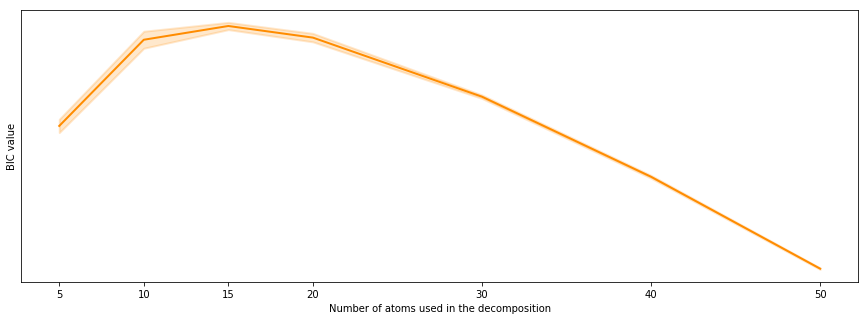
\includegraphics[scale=0.5]{parameterresearch.png}
\caption{Curve of the \texttt{scoring\_function} values (refined BIC) w.r.t. the number of atoms used for the decomposition. To an higher value corresponds a better model for the dataset. In this case the best model is the one with 15 atoms in the dictionary.}
\label{bic}
\end{figure}
%
%
%
%
%
\section{Appendix: interchangeability of the penalties} \label{penalty change}
With DALILA trying different penalties on the same dataset requires only few lines of code. 

For example suppose we have the right number of atoms (with the dataset we use is 7) in which to decompose the dataset and that, some oracle, told us the perfect regularisation parameters for each penalty on that dataset. Then we may want to try different sparsifications on the coefficients to see which one better approximates the original signal. We tried \texttt{L1Penalty}, \texttt{L0Penalty} and \texttt{ElasticNetPenalty}.

\begin{lstlisting}[language=Python]
import numpy as np

from dalila.dictionary_learning import DictionaryLearning
from dalila.dataset_generator import synthetic_data_non_negative
from dalila.penalty import L1Penalty, L0Penalty, ElasticNetPenalty

X, D, C = synthetic_data_non_negative()

estimator = DictionaryLearning(k=7, coeff_penalty=L1Penalty(0.01), non_negativity="both")
estimator.fit(X)
C_l1, D_l1 = estimator.decomposition()
error_l1 = estimator.reconstruction_error()

estimator = DictionaryLearning(k=7, coeff_penalty=L0Penalty(3), non_negativity="both")
estimator.fit(X)
C_l0, D_l0 = estimator.decomposition()
error_l0 = estimator.reconstruction_error()

estimator = DictionaryLearning(k=7, coeff_penalty=ElasticNetPenalty(0.01, 0.1, 0.7), non_negativity="both")
estimator.fit(X)
C_en, D_en = estimator.decomposition()
error_en = estimator.reconstruction_error()
\end{lstlisting}
After the execution of this piece of code the comparison between the results is straight-forward and you can notice that the effort is minimal. 

\section{Appendix: addition of a new penalty} \label{new penalty}
DALILA allows to easily introduce new customised penalties for the optimisation of dictionary learning or representation learning. We want to underline that, even if the implementation steps are easy, the function that computes the proximal mapping has to be correct and no theoretical inconsistencies should be present. The behaviour is otherwise unpredictable.  \\


The first step is the import of the super-class Penalty that our new penalty has to extend. We also import other things that we need later.
\begin{lstlisting}[language=Python]
from dalila.representation_learning import RepresentationLearning
from dalila.penalty import Penalty
import numpy as np
\end{lstlisting}
The implementation of the new class, besides the construction, has to expose the method \texttt{apply\_prox\_operator} that is the one called during the minimisation. In this method the prox operator is implemented. 
\begin{lstlisting}[language=Python]
class NewPenalty(Penalty):
    
    def __init__(self, regularization_parameter):
        self.regularization_parameter = regularization_parameter
	
	  # x is the matrix on which apply the prox
	  # gamma is the gradient descent step
    def apply_prox_operator(self, x, gamma): 
        # if you are declaring a real penalty
        # change the implementation and 
        # transform x according to your penalty
        return x

\end{lstlisting}
Once we have declared the penalty, in this case a penalty that does nothing, we put it into the representation learning procedure. 
\begin{lstlisting}[language=Python]
fake_data = np.random.rand(50,50)
fake_dictionary = np.random.rand(5, 50)
estimator = RepresentationLearning(fake_dictionary, penalty=NewPenalty(5))
estimator.fit(fake_data)
\end{lstlisting}\vspace{0.2cm}
It is also possible to use the parameter research procedures with the new penalty provided that we also overwrite the method \texttt{make\_grid} since the searching function assumes it exists. We here show a basic example of how it can be implemented, one may want to vary the interval or the sampling procedure. 
\begin{lstlisting}[language=Python]
class NewPenalty(Penalty):
   
	  # ..as above..
        
    def make_grid(self, low=0.001, high=1, number=10):
		# possible regularization parameters to analyse        
        values = np.linspace(low, high, number)
        l = []
        # the list has to be composed of NewPenalty objects
        for (i, v) in enumerate(values):
            l.append(NewPenalty(v))
        return l
\end{lstlisting}
Again we show that it is usable right away without further code.
\begin{lstlisting}[language=Python]
from dalila.parameters_research import tune_parameters_RL
estimator = RepresentationLearning(fake_dictionary, penalty=NewPenalty(5))
gscv = tune_parameters_RL(fake_data, estimator, coeff_penalty_range=(0.1, 1, 3))
\end{lstlisting}



\end{document}
